\chapter{Introduction}
\label{sec:introduction}

This thesis revolves around measurements involving a two photon final state.
The diphoton decay channel has been one of the two decay modes that led to the
first observation of the Higgs boson~\cite{cms_atlas_hgg_comb}. The same
final state provide a probe to test models describing new physics such as quantum gravity
effective theories based on extra dimensions or Super Symmetry (SUSY) models with an extended
Higgs sector. The nature of the photon restrict the
particles that can decay to a two photon system to bosons with either
spin equal to zero or spin strictly greater than one~\cite{landau,yang}.
A search for beyond the standard model (BSM) resonances, performed with p-p collision data collected by the CMS experiment,
is presented in Chapter~\ref{chapter:diphotons} together with the description of the calibration procedure (Chapter~\ref{chapter:ecal}
of the detector component that contributes the most to the detection of photons in CMS (i.e. the electromagnetic calorimeter).

Measurement involving a diphoton system in the final state also includes the measurement of the Higgs boson self coupling
through di-Higgs production in p-p collisions. This standard model process is extremely rare, thus its observation is
only possible with a large dataset of p-p collisions. Such dataset will be produced during the high luminosity
phase of LHC (HL-LHC), in Chapter~\ref{chapter:upgrade} the major goal and challenges of are described together with
the preliminary studies to incorporate the time information into the event reconstruction of CMS as a way to meet
the performance needed to fully exploit data collected in the high luminosity phase.

In the following sections the theoretical framework of fundamental interaction is briefly introduced.
The main focus is describe the standard model, the phenomenology of hadronic collisions and the models
which gives rise to a BSM resonant diphoton production.

\section{The standard model of particle physics}
During the 20th century the development of new technologies enabled experimental
physicist to explore matter at the atomic and sub-atomic levels. At these levels
is possible to explore the building blocks of matter and the interactions between them.

A theory has been constructed during the past century which describes and predicts
a large part of the natural processes that are know today. The Standard Model of particle physics (SM)
describes in coherent way three types of interactions between sub-atomic particles:
the behavior of electromagnetic, weak and strong interaction at a quantum level is
addressed by the SM, this in fact allows us to describe a variety of phenomena with a
single mathematical framework.

The SM is build upon relativistic quantum field theory. The constituents of matter are particles
with half-integer spin that follow the Fermi-Dirac statistic while the interactions are mediated by
integer spin particles which follow Bose-Einstein statistic. Is common to refer at the first group as
fermions and to the second as bosons. Tables \ref{tab:fermions} and \ref{tab:bosons}
show the fermions and bosons described by the SM and their
main properties. 

\begin{table}[ht]
  \begin{center}
    \begin{tabular}{|c|cc|cc|cc|c|c|}
    \hline
    & \multicolumn{2}{c|}{$1^{\textnormal{st}}$ gen.}
    & \multicolumn{2}{c|}{$2^{\textnormal{nd}}$ gen.}
      & \multicolumn{2}{c|}{$3^{\textnormal{rd}}$ gen.}
      & $Q$
      & Colour Charge \\
    \hline
    \hline
    \multirow{2}{*}{leptons} &
    \textnu$_{\textnormal{e}}$            & \small{$\sim 0$} &
    \textnu$_{\textnormal{\textmugreek}}$ & \small{$\sim 0$} &
    \textnu$_{\textnormal{\texttau}}$     & \small{$\sim 0$} &
    0 & 0 \\
    &
    e            & \small{$511 \mathrm{keV}/\mathrm{c}^2$}   &
    \textmugreek & \small{$105.7 \mathrm{MeV}/\mathrm{c}^2$} &
    \texttau     & \small{$1.777 \mathrm{GeV}/\mathrm{c}^2$} &
    -1 & 0 \\
    \hline
    \multirow{2}{*}{quarks} &
    u & \small{$1.7-3.1\mathrm{MeV}/\mathrm{c}^2$}         &
    c & \small{$1.29^{+0.05}_{-0.11}\mathrm{GeV}/\mathrm{c}^2$}  &
    t & \small{$172.9^{+1.1}_{-1.1}\mathrm{GeV}/\mathrm{c}^2$} &
    2/3 & $r,g,b$ \\
    &
    d & \small{$4.1-5.7\mathrm{MeV}/\mathrm{c}^2$} &
    s & \small{$100^{+30}_{-20}\mathrm{MeV}/\mathrm{c}^2$} &
    b & \small{$4.19^{+0.18}_{-0.06}\mathrm{GeV}/\mathrm{c}^2$} &
    -1/3 & $r,g,b$  \\
    \hline
    \end{tabular}
  \end{center}
  \caption{Spin-$\tfrac{1}{2}$ fermions masses, electric charges (in units of the positron charge) and color charges~\cite{PDG}.}
  \label{tab:fermions}
\end{table}

\begin{table}[ht]
  \begin{center}
    \begin{tabular}{|c|c|c|c|}
    \hline
    & Mass (GeV)
    & $Q$
    & Colour Charge \\
    \hline
      \hline
      Photon ($\gamma$) & 0 & 0 & 0 \\
      Gluon ($g$) & 0 & 0 & $r,g,b$ \\
      W & $80.385 \pm 0.015$ & $\pm 1$ & 0 \\
      Z$^0$ & $91.188 \pm 0.002$ & 0 & 0 \\
    \hline
    \end{tabular}
  \end{center}
  \caption{Spin-1 bosons masses and charges~\cite{PDG}.}
  \label{tab:bosons}
\end{table}

Fermions differ from each other by mass and coupling to the force carriers, a charge is associated
to each interaction so a total of four values is used to identify a fermion: three charges and one mass.
Fermions with non-null color charge are named quarks and interact strongly with each other through the exchange
of gluons, the strong force carriers. The other fermions, called leptons, that are insensitive to
the strong force interacts only electroweakly.

At the core of the SM there is the concept of gauge invariance.
Since Maxwell's unification of electric and magnetic interactions, gauge invariance
has played a strategic role in the description of the fundamental interaction of matter.
The requirement of a symmetry in the Lagrangian of a theory accounts for conservation of
charges, via the Noether's theorem.
The mediators of the interaction are introduced to preserve the conservation of
the free particle Lagrangian under the gauge transformation of the type $\psi \to e^{i\alpha}\psi$, where
$\psi$ is a generic fermion field.

In these terms the SM is based on a group of three symmetries $SU_C(3)\times SU_L(2) \times U_Y(1)$.
The three symmetries are related to three local gauge invariances of the Lagrangian that describes the interaction
between the particles described above.

$SU_C(3)$ is related to the strong interaction mediated by the massless gluons. It conserves the colour charge
carried by quark and gluons which appear as colour triplets under $SU_C(3)$ transformation.
The experimental evidence is that coloured particles cannot propagate freely.
Quarks and gluons are only observed in bound states as mesons $q\bar{q}$ and barions $qqq$.
This behaviour is known as
asymptotic free, i.e. he coupling is asymptotically weaker as energy increases and distance decreases
and conversely it becomes stronger at larger distances.

The $SU(2)_{L} \times U(1)_{Y}$ group is associated to electroweak interactions, which are the
unified description of electromagnetism and weak interactions. The long-range electromagnetic
interaction is mediated by the massless photon ($A_{\mu}$ field), while the short-range weak force carriers are the
massive $W^{+}$, $W^{-}$ and $Z^{0}$ bosons. Unlike the gluons the electroweak mediators
are not the direct fields introduced to preserve the gauge invariance but instead are combinations
of them. In particular the $W_{\mu}^3$ and $B_{\mu}$ introduced respectively for the $SU_L(2)$ and $U_Y(1)$ symmetries
are mixed to obtain the physical $A_{\mu}$ and $Z_{\mu}$ fields:
\[
\begin{split}
  W_{\mu}^{\pm} & = \frac{1}{\sqrt{2}}\left(W_{\mu}^{1}\mp i W_{\mu}^{2}\right) \\
  \left(
  \begin{array}{c}
  A_{\mu} \\ Z_{\mu}
  \end{array}
  \right)
  & =
  \left(
  \begin{array}{cc}
  \cos\theta_{W} & \sin\theta_{W} \\
  -\sin\theta_{W} & \cos\theta_{W}
  \end{array}
  \right)
  \left(
  \begin{array}{c}
  B_{\mu} \\ W_{\mu}^{3}
  \end{array}
  \right) \quad ,
\end{split}
\]

where Weinberg mixing angle ($\theta_W$) has been measured at the Z-pole at LEP as
$sin^2(\theta_W) = 0.23153 \pm 0.00016$.

The mixing is also reflected in the conserved charges for which the following relation holds:
\[
  Q = T_3 + \frac{Y}{2}
\]
where $Q$ is the electric charge, $Y$ the $U_Y(1)$ hypercharge and $T_3$ is the third component of the weak
isospin $T$ conserved by the $SU_L(2)$ symmetry.

The $W^{\pm}$ bosons couple only to the left-handed components $\psi_{L}$ of the fermion fields,
while the $Z^{0}$ and $\gamma$ bosons couple to both $\psi_L$ and
$\psi_R$, thus leading to the observed parity-violation phenomena of weak interactions.
The asymmetry between right and left handed fermions also forbids the inclusion of a
Yukawa mass terms into the standard model Lagrangian since such a term would not be invariant under $SU_L(2)$
transformation.
This fact has an remarkable consequence: the three generation of leptons and quarks summarized
in Table~\ref{tab:fermions} are identical from the perspective of the strong and electroweak interactions
since they only differ for their masses.
Table~\ref{tab:charges} summarize the charges for all known fermions families: 
\begin{table}[ht]
  \begin{center}
    \begin{tabular}{|c|c|c|c|c||c|c|c|c|c|}
      \hline
      & $T$
      & $T_3$
      & $Y$
      & $Q$
        &
      & $T$
      & $T_3$
      & $Y$
      & $Q$ \\
          \hline 
      $l_L$ & $1/2$ & $-1/2$ & $-1$ & $-1$  & $q_L^{down}$ & $1/2$ & $-1/2$ & $1/3$ & $-1/3$ \\      
      $\nu_L^l$ & $1/2$ & $1/2$ & $-1$ & $0$  & $q_L^{up}$ & $1/2$ & $1/2$ & $1/3$ & $2/3$ \\
      $l_R$ & $0$ & $0$ & $-2$ & $-1$  & $q_R^{down}$ & $0$ & $0$ & $4/3$ & $2/3$ \\
      $\nu_R^l$ & $0$ & $0$ & $0$ & $0$  & $q_R^{up}$ & $0$ & $0$ & $-2/3$ & $-1/3$ \\
      \hline
    \end{tabular}
  \end{center}
  \caption{Charges (quantum numbers) of leptons (left) quarks (right).}
  \label{tab:charges}
\end{table}

Notably the right-handed neutrino is sterile in the standard model, i.e. it does not couple to
any of the three forces carriers. 

The standard model described above has proven over the years to be remarkably accurate in describing and
predicting the interaction of matter at the quantum level.
However there a number of processes observed in Nature that cannot be explained by the otherwise complete model:
\begin{itemize}
\item Cosmological dark matter.
\item Matter-antimatter asymmetry.
\item Neutrinos oscillations and masses.
\end{itemize}
To name some of them. Furthermore the SM lacks a quantum description of gravity and also requires
a ``fine tuning'' (more later) of some of its parameters.

These issue are addressed by several models extending the SM, most of them predicts the existence of new particles
(arising from the same gauge invariance request explained above) that could be observed either through the
products of their decay or from virtual interference with standard model interactions.
In both cases hadronic collision offers a unique way to test such models providing both the possibility
to produce them or infer their existence from precise measurement of the standard model parameters.

\section{Proton-proton collisions}
The precise measurement of the electroweak sector at the LEP and SLC electron-positron colliders and the discovery of the top
quark at Tevatron proton-antiproton collider, the yet to be observed Higgs boson and the search for BSM physics led
to the construction of the Large Hadron Collider (LHC).

Hadronic colliders, in the context of high energy physics, are great tools for discoveries since
protons are composite particles and thus both the hard scattering energy and its nature are not restricted by
the machine parameters but covers a wide range of possibilities.
The inner structure of the proton have been extensively studied in recent years at the electron-proton collider HERA
at DESY~\cite{hera}. The proton, as all other barions, is made of three ``valence'' quark surrounded by a ``sea''
of gluons and quark-antiquark pairs. Quarks and gluons in this context are referred to as partons. 
This qualitatively description is translated into a quantitative description by the DGLAP equations using perturbative
quantum chromodinamics (QCD)~\cite{altarelli_parisi,gribov,dokshitzer}.
The probability to find a parton carrying a fraction ``$x$'' of the total proton momentum
is described by the parton density functions (PDFs).
As shown in Figure~\ref{fig:pdfs} the valence quark dominates over the sea partons for $x>0.1$.
The PDFs depends on the momentum transferred in the scattering process, in particular for
larger values of momentum transfer $\mu^2$ the gluon PDFs dominates over the valence quark. For this reason
``gluon-fusion'' initiated processes dominates at LHC.

\begin{figure}
  \centering
  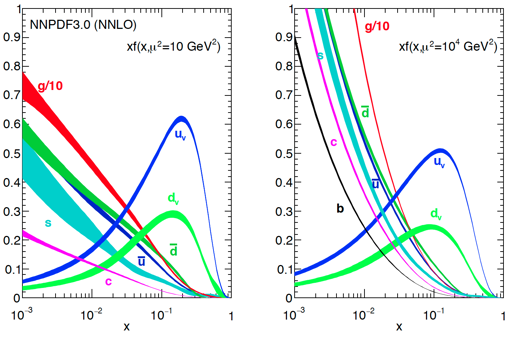
\includegraphics[width = 0.7\textwidth]{figures/introduction/pdfs.png}
  \caption{
    Distributions of $x$-times the unpolarized parton distribution function $f(x)$
    obtained in the NNPDF 3.0 global analysis at the scales of $\mu^2 = 10 \mathrm{GeV}^2$ (left) and
    $10^4 \mathrm{GeV}^2$ (right) at $\alpha_s(M_Z) = 0.118$~\cite{pdfs}.}
  \label{fig:pdfs}
\end{figure}

the perturbative QCD well describes the hard part of the hadronic collisions and the emission of
energetic quark and gluons as initial and final state radiation,
while the description of the formation of bounded QCD states from bare quark and gluons involves non-perturbative, low $\mu^2$
processes generally called ``hadronization''. 

The hadronization of quark and gluons coming from high $\mu^2$ processes (hard scattering) gives rise
to a jet of collimated hadrons , which are usually reconstructed in collider experiments as energy clusters.
The kinematic of a jet is directly linked to the one of the original quark or gluon, allowing the reconstruction
of the hard scattering.

An hard scattering usually only involves a parton from each colliding proton, the other partons interact at low $\mu^2$
(soft interactions) giving rise to the so called ``underlying event'' i.e. particles of low transverse momentum $p_T$
produced in conjunction with the boosted products of the hard interaction.

\section{Extra dimensions and the hierarchy problem}
The hierarchy problem is a common way to, within the high energy physics community, refer to the large
discrepancy arising between the effective value of a constant and the fundamental value it has
in the Lagrangian that describes the dynamics of the model under consideration

An example in SM is given by higher order corrections to the Higgs boson mass. These includes loops of
massive particles which for one fermion give a correction expressed as:
\[
  \Delta M_H^2 = \frac{\lambda_f^3}{4\pi}(\Lambda^2 + m_H^2)
\]
If one imposes a cutoff at a scale $\Lambda$ close to the Planck mass ($M_{Pl}\sim 10^{19}$GeV) a cancellation
of the radiative correction for this fermion loops occurs for $m_H = 246$GeV and $(m_H/Lambda)^2 \sim 10^{34}$
(here $m_H$ the fundamental Higgs boson mass equal to the vacuum expectation value for the Higgs field and
$\Delta M_H$ represent the correction that gives the observed Higgs boson mass).

Is evident that such a small value of $(m_H/Lambda)^2$ represent a ``fine-tuning'' of the theory which otherwise
would give rise to an incredibly huge Higgs boson mass (compared to all other particles in the standard model).
The ``fine-tuning'' cannot be explained within the framework of the SM alone,
however extra dimension models offer a solution to this fine tuning.

Extra dimension models (ED) were introduced by Kaluza-Klein~\cite{kk} in attempt to unify the electromagnetism
with the description of gravity given by Einstein's general relativity.
The general idea is that existence of a multidimensional space-time with at least 4 space dimensions
and one time dimension. This space-time is an extension of the four-dimensional Minkowsky space and the weakness of
the gravity interaction is explained by its propagation through the extra dimensions.

Extra dimension as solution for the hierarchy problems were first proposed
by Arkani, Dimopoulos and Dvali (thus the name ADD model)~\cite{ADD}.
The existence of $n$ additional spatial dimensions, compactified with
average radius $R$, produces an effective Planck mass in our four-dimensional world that is related to the true
Planck Mass by: $M_{Pl}^2 \sim M_{Pl(4_n)}^{n+2}R^n$. It is therefore possible, with appropriate values for $n$
and $R$, that the true value of the Planck scale ($M_{Pl(4_n)}$) could be on the order of the electroweak scale,
thus solving the SM hierarchy problem, while still producing the much larger apparent Planck
scale that we observe in our four-dimensional world.

Randall and Sundrum (RS) proposed an alternative model~\cite{RS}, with just one additional dimension
that has a warped geometry, described by curvature parameter $k$. The extra dimension $y$
is wrapped, meaning that it is curled up to a circle with a finite radius $r_c$ and curvature parameter $k$.
The five-dimensional space-time metric is given by:
\begin{equation}
  ds^2 = e^{-2ky}\eta_{\mu\nu}dx^{\mu}dx^{\nu} + d^2y 
\end{equation}
\label{eq:extra_dim_metric}

From the left sketch of Figure ?? it is visible that the opposite coordinate points on the circle need to be
identified with each other, imposing the boundary conditions of $y = 0$ and $|y| = \pi r_c = L$.
The two boundary conditions determine the warp factor of Equation~\ref{eq:extra_dim_metric}:
\[
  \frac{e^{-k|y(L)|}}{e^{-k|y(0)|}} = e^{-2kr_c}
\]



Values of $kr_c \sim 11-12$ gives an observed Planck scale of the order of few TeV
From the point of view of a four-dimensional observer, a fundamental mass
parameter $m_0$ defined on the SM brane in the full 5D theory will appear as a physical mass
m = e − kr c π m 0 . In this model, solving the hierarchy problem requires that the fundamental
mass should be m 0 ∼ M Pl and the observed mass should be TeV-scale. Because of the exponen-
tial warp factor, this large hierarchy can be naturally generated if kr c ≈ 11 − 12.

\section{Extra dimension signatures in proton-proton collisions}
In both the ADD and RS models the perturbative KK expansion of the five-dimensional metric
gives origin to an infinite number of four-dimensional spin-2 fields (gravitons). Together with
the massless spin-2 boson associated to gravity an infinite number of massive gravitons are predicted to exist
at masses that are of the order of the TeV.
In the ADD model the four-dimensional massive states
are closely spaced and thus produce a degenerate spectrum when they decay into SM particles.
RS model instead predicts the existence of well separated mass states of which only the first one has a mass
within the energy reach of LHC.

The RS-like models can be further categorized depending on how much the SM fields propagates into the five-dimensional
space-time. 

\section{Standard model diphoton production}
\label{sec:sm_dipho_prod}
The main background for the search of BSM resonances decaying to two photons is the standard model production
of photon pairs. Photon pairs production is possible through leading order processes involving two
initial state quarks $q\bar{q}\to\gamma\gamma$. Higher order terms in perturbative QCD also contribute to
the total production cross section and the corresponding Feynman diagrams are illustrated in Figure~\ref{fig:nlo_dipho}.
